\chapter{Aufgabe 5}

\section{Teil 1}


\textit{Wie heißt die Schaltung eines Schaltwerkes, das aus Eingangs- und
Ausgangsschaltnetz und einem Speicher besteht (Folgezustände werden
aus dem aktuellen Zustand und dem Eingangsschaltnetz ermittelt, die
Ausgangsbelegung soll sich synchron zum Takt ändern)?}\\

\noindent
Es handelt sich wohl um das \textbf{taktzustandsgesteuerte RS-Flipflop} (\cite[65 f.]{ES1}), ein RS-Flipflop mit Torschaltung $C$ (\textit{Clock}), die nur dann Signale zum Flipflop durchlässt, wenn $C$ auf $1$ liegt.\\
\textit{Bollenbacher und Liell} weisen darauf hin, dass in der Praxis \textit{flankengesteuerte} Flipflops bevorzugt werden,  ``da sie nur zu einem \textit{genau definierten} Zeitpunkt (sehr kurze Zeit) die Eingangsinformation übernehmen `` (\textit{ebd.}, Hervorhebung i.O.).\\

\noindent
(Will man den illegalen Zustand $R=1, S=1$ verhindern, nutzt man \textit{D-Flipflops} als Erweiterung von RS-Flipflops. $R=1, S=1$ würde - grob gesagt - bedeuten, dass der Speicherinhalt dieser Kippstufe gleichzeitig \textit{gesetzt} und \textit{zurückgesetzt} wird - theoretisch ist dieser Zustand \textit{undefiniert}.
D-Flipflops verhindern dies, indem es einen aktiven Eingang gibt, der negiert auf einen weiteren Eingang geleitet wird - so kann nie gleichzeitig derselbe Eingangspegel anliegen.
Zusätzlich besitzt der D-Flipflop noch eine Torschaltung $C$, die die Weitergabe des Eingangssignals steuert (vgl.~\cite[69]{ES1}, wo D-Flipflops für den Aufbau eines synchronen Schaltwerks genutzt werden).)

\section{Teil 2}

\textit{Ergänzen Sie in der Tabelle die Folgezustände.}\\

\noindent
Der Lösungsvorschlag zu Aufgabe 5.2 ist in Tabelle~\ref{tab:zustandsfolgetabelle} angegeben.\\
Bei der Lösung sind $z_1^+, z_0^+$ die Eingaben für die Motorsteuerung, die aus zwei Eingängen \texttt{ML}, \texttt{MR} besteht - wie wir sehen werden, wird für die Ausgabe - also die Motoreingänge - kein separates Schaltnetz benötigt.\\
Ist \texttt{ML} = 1, wird die Drehrichtung des Motors auf Linksbetrieb gestellt, bei \texttt{MR} = 1 auf Rechtsbetrieb.\\
Der Zustand \texttt{ML} = 1 $\land$ \texttt{MR} = 1 ist undefiniert.\\
Befindet sich das System im Zustand Messen, sind \texttt{ML} = 0 sowie \texttt{MR} = 0.

\begin{table}[h!]
    \centering
    \setlength{\tabcolsep}{0.5em}
    \def\arraystretch{1.5}
    \begin{tabular}{|c|c|c|c||c|c||c|c||l|}
        \hline
        \textbf{$z_1$} & \textbf{$z_0$} & \textbf{L} & \textbf{R} & \textbf{$z_1^+$} & \textbf{$z_0^+$} & \texttt{ML} & \texttt{MR} & Anmerkung \\
        \hline
        \hline
        0 & 0 & 1 & 0 & 0 & 1 & 0 & 1 & Messen $\land$ LS L offen $\rightarrow$ nach rechts\\ \hline
        0 & 0 & 0 & 1 & 1 & 0 & 1 & 0 & Messen $\land$ LS R offen $\rightarrow$ nach links \\ \hline
        \hline
        0 & 1 & 1 & * & 0 & 1 & 0 & 1 & nach rechts $\land$ LS L offen $\rightarrow$ nach rechts \\ \hline
        0 & 1 & 0 & * & 0 & 0 & 0 & 0 & nach rechts $\land$ LS L schließt $\rightarrow$ messen \\ \hline
        \hline
        1 & 0 & * & 1 & 1 & 0 & 1 & 0 &  nach links $\land$ LS R offen $\rightarrow$ nach links \\ \hline
        1 & 0 & * & 0 & 0 & 0 & 0 & 0 &  nach links $\land$ LS R schließt $\rightarrow$ messen \\
        \hline
    \end{tabular}
    \caption{Lösungsvorschlag für die Zustandsfolgetabelle aus Aufgabe 5.2. Die Abkürzung ``LS`` ist aus der Aufgabenstellung übernommen und steht für ``Lichtschranke``. Die Zustände ``offen`` bzw. ``schließt`` stehen für eine nicht verdeckte bzw. verdeckte Lichtschranke. (Quelle: eigene)}
    \label{tab:zustandsfolgetabelle}
\end{table}

\section{Teil 3}

\textit{Bestimmen Sie die KV-Diagramme und die Funktionsgleichungen des
Eingangsschaltnetzes.
Versuchen Sie, die Schaltfunktionen zu vereinfachen, indem Sie benachbarte Eins-Felder zu Blöcken zusammenfassen. Markieren Sie diese
Blöcke im KV-Diagramm.}\\

\noindent
\subsection*{Funktionsgleichungen}

Die Funktionsgleichung für $z_1^+$ ist in~\ref{eq:dnf_z1} als DNF angegeben, entsprechend für $z_0^+$ in~\ref{eq:dnf_z0}.\\
Die \textit{Don't-Care-Eingaben} wurden dabei berücksichtigt.

\begin{equation}\label{eq:dnf_z1}
\begin{alignat}{3}
    z_1^+ =\ &(\neg z_1 \ \land \neg z_0 \ \land \neg L \ \land \phantom{\neg} R)\ \lor &&  \\
    &(\phantom{\neg} z_1 \ \land \neg z_0 \ \land \phantom{\neg} L \ \land \phantom{\neg} R)\ \lor &&  \\
    &(\phantom{\neg} z_1 \ \land \neg z_0 \ \land \neg L \ \land \phantom{\neg} R)
\end{alignat}
\end{equation}

\begin{equation}\label{eq:dnf_z0}
\begin{alignat}{3}
    z_0^+ =\ &(\neg z_1 \ \land \neg z_0 \ \land \phantom{\neg} L \ \land \neg R)\ \lor &&  \\
    &(\neg z_1 \ \land \phantom{\neg} z_0 \ \land \phantom{\neg} L \ \land \phantom{\neg} R)\ \lor &&  \\
    &(\neg z_1 \ \land \phantom{\neg} z_0 \ \land \phantom{\neg} L \ \land \neg R)
\end{alignat}
\end{equation}

\subsection*{KV-Diagramme}

Das KV-Diagramm für $z_1^+$ ist in~\ref{fig:kv_z1}, für $z_0^+$ in~\ref{fig:kv_z0} dargestellt.\\
Basierend darauf kann für $z_1^+$ wie folgt vereinfacht werden (siehe~\ref{eq:z1_min}):

\begin{equation}\label{eq:z1_min}
\begin{alignat}{3}
    z_1^+_{\text{min}} =\ &(\neg z_0 \ \land \neg L \ \land \phantom{\neg} R)\ \lor   \\
    &(\phantom{\neg} z_1 \ \land \neg z_0 \ \land \phantom{\neg} R)
\end{alignat}
\end{equation}

\noindent
Für $z_0^+$ ergibt sich (siehe~\ref{eq:z0_min}):

\begin{equation}\label{eq:z0_min}
\begin{alignat}{3}
    z_0^+_{\text{min}} =\ &(\neg z_1 \ \land \phantom{\neg} L \ \land \neg R)\ \lor &&  \\
    &(\neg z_1 \ \land \phantom{\neg} z_0 \ \land \phantom{\neg} L)
\end{alignat}
\end{equation}

\begin{figure}
    \centering
    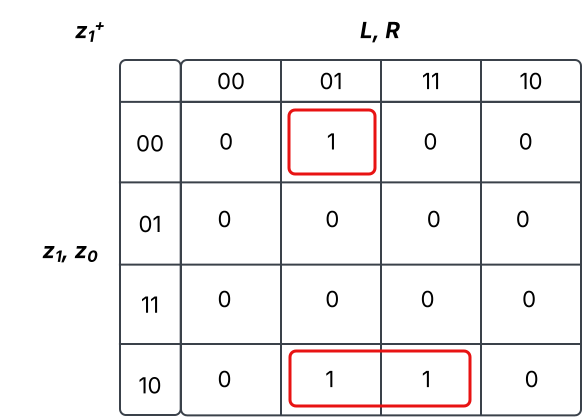
\includegraphics[scale=0.5]{aufgabe 5/img/kv_z1.svg}
    \caption{KV-Diagramm für $z_1^+$ aus Aufgabe 5.3.  (Quelle: eigene)}
    \label{fig:kv_z1}
\end{figure}

\begin{figure}
    \centering
    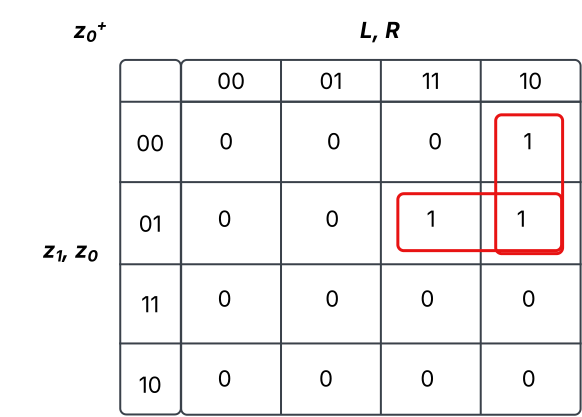
\includegraphics[scale=0.5]{aufgabe 5/img/kv_z0.svg}
    \caption{KV-Diagramm für $z_0^+$ aus Aufgabe 5.3.  (Quelle: eigene)}
    \label{fig:kv_z0}
\end{figure}

\noindent
Das synchrone Schaltwerk ist in Abbildung~\ref{fig:synch} dargestellt.

\begin{figure}
    \centering
    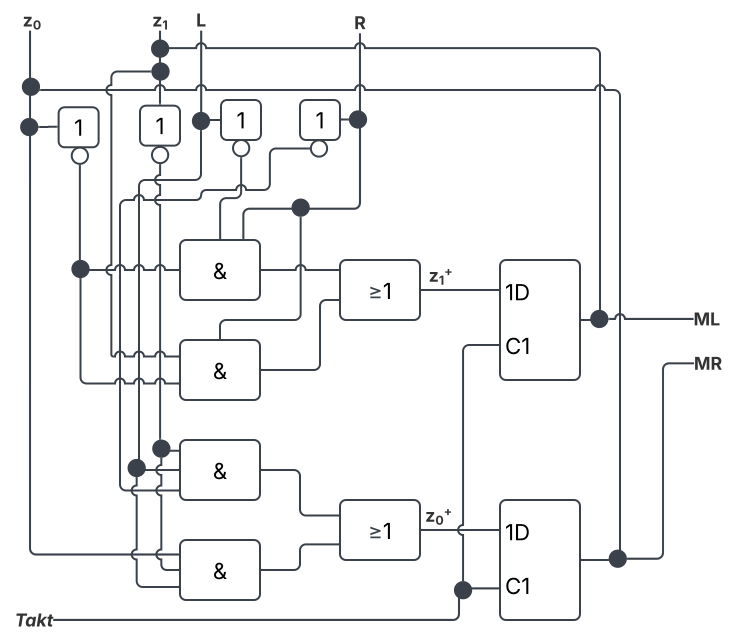
\includegraphics[scale=0.5]{aufgabe 5/img/synch.svg}
    \caption{Synchrones Schaltwerk für die Motorsteuerung aus Aufgabe 5.3. Eingezeichnet sind die Ausgaben \texttt{MR} / \texttt{ML}, die kein separates Schaltnetz benötigen, da sowohl $z_1^+ &= \texttt{ML}$ als auch $z_0^+ &= \texttt{MR}$ gilt (s. Tabelle~\ref{tab:zustandsfolgetabelle}). (Quelle: eigene)}
    \label{fig:synch}
\end{figure}

\section{Teil 4}

\textit{Bestimmen Sie die Funktionsgleichungen des Ausgangsschaltnetzes und
tragen Sie diese in die Schaltung ein.}\\

\noindent
Ein separates Schaltnetz für die Ausgänge \texttt{ML} / \texttt{MR} ist nicht nötig, da sie den Zuständen $z_1^+$ / $z_0^+$ entsprechen:

\begin{equation}\notag
    \begin{split}
        z_1^+ &= \texttt{ML} \\
        z_0^+ &= \texttt{MR}
    \end{split}
\end{equation}
